\documentclass{report}
%----- PACKAGES------------- 
\usepackage[T1]{fontenc}
\usepackage[utf8]{inputenc}
\usepackage{amsmath,amssymb,amsthm}
\usepackage[shortlabels]{enumitem}

\usepackage{graphics}
\usepackage{graphicx}
\usepackage{tikz-cd}
\usepackage{tikz}
\usetikzlibrary{backgrounds,decorations.pathreplacing,patterns,positioning,arrows.meta}
\usepackage{hyperref}
\usepackage{multicol}
\setlength{\columnsep}{5cm}
\usepackage{soul}
\usepackage{xcolor}
%----commands -------------

\newcommand{\NN}{\mathbb{N}}
\newcommand{\ZZ}{\mathbb{Z}}
\newcommand{\QQ}{\mathbb{Q}}
\newcommand{\RR}{\mathbb{R}}
\newcommand{\CC}{\mathbb{C}}



%----Theoremstyles------


\theoremstyle{plain}
\newtheorem{theorem}{Théorème}
\newtheorem{lemme}[theorem]{Lemme}
\newtheorem*{proposition}{Proposition}
\newtheorem{corollary}[theorem]{Corollary}


\theoremstyle{remark}
\newtheorem*{remarque}{Remarque}

\theoremstyle{definition}
\newtheorem*{definition}{Définition}
\newtheorem*{definitions}{Définitions}
\newtheorem*{observation}{Observation}
\newtheorem{notation}{Notation}
\newtheorem*{exemple}{Exemple}
\newtheorem{exercice}{Exercice}
\newtheorem*{Exercicesup}{Exercice supplémentaire}


%--- Structure---

\usepackage{titlesec}



\newcommand{\exo}[1]{\noindent \textbf{Exercice #1}}
\newcommand{\solution}{\noindent \textbf{Solution}}
\newcommand{\ajd}[1]{\noindent \textbf{Au programme:} #1}





\title{Box Problem}
\author{Dries Rooryck}

\begin{document}
\maketitle
\chapter{The box problem }
\section{Explanation of the game}
In a simplified version of the TV gameshow, imagine having ten  carboard boxes aligned in a row. Each box contains between 1 and 10 euros. The boxes are mixed up and \textit{randomly distributed}, meaning one does not know what the probability is of having a certain amount of money in each box.\\
Every round, you open a box. When you open a box, you have two options:
\begin{itemize}
\item(i) You take the money that you find in this box, and the round ends. 
\item(ii) You throw away the box and choose a new box from the remaining ones. 
\end{itemize}
If you choose the box with the largest sum of money, you win. However, you lose if there was another box with more money.\\

What could be a good strategy to win the most rounds?

\section{Computer Simulation}
I firstly coded a simulation of the game on javascript. This code would simulate a game with a strategy that the user could input. I could then run this simulation $10^5$ times, and calculate how many times i won and lost the round. With this information i could calculate a 'winrate' for a specific strategy. \\
With a computer script in place, i could now automatize many aspects of the simulation, such as
\begin{itemize}
\item the number of boxes, instead of being restricted to 10.
\item the distribution of money(gaussian, uniform, random).
\item Calculating the average biggest amount of money, which i will come back to later
\item Count the amount of boxes with different amounts of money, in order to test the distribution
\end{itemize}

\section{Uniform Distribution}



Firstly, I considered a special case.\\
It can be at first quite counter-intuitive to think of a 'random' distribution of the amount of euros. One tends to imagine filling each box uniformly. An analogy for a uniform distribution is the roll of a fair 10 sided die. What a 'random' distribution means, is that the die is not fair, and its dimensions (fairness) are not known.

 Instead of having this random distribution of money, i first considered the money to be uniformly distributed per box. This means that every box has the same chance of having 1-10 euros, continuing the analogy of a fair 10-sided die. \\

Now we can try to find a good strategy only for this uniform distribution.

\section{Lower Bound Pick}

The first strategy that seemed logically intuitive to me, was what one could call a 'lower bound pick'. You choose a lower boundary of how much money it will take for me to pick the box, and take anything above it. For example, if the lower boundary were 6, one would take the first box that has more than 6 dollars inside.\\ 
After simulating this strategy in my code environment, I observed that a lower boundary of 8 (picking a box when it has 9 or 10 dollars) produced the highest winrate, of about 68,74 \% \\
Here is a plot of the lower boundary chosen on the x-axis, and the consequently observed winrate on the y-axis.\\
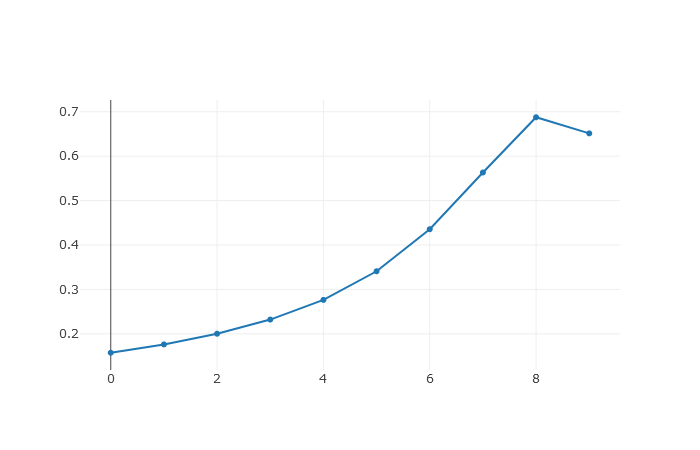
\includegraphics[scale=0.4]{newplot.png}

\pagebreak

\subsection{Theory}
The next step was to find a mathematical theorem behind the observed winrate for each lower boundary.

Let us consider the lower boundary $b = 8$\\

One could win in two possible with two values, 9 or 10 dollars, in 10 different boxes $i$ \\
Example with a fixed value(dollars = 9) and fixed box (i=3):\\
The probabilty of winning with \textbf{9 dollars in the third box} is made up of three constituent parts:\\

\begin{enumerate}

\item P(The 3rd box contains 9 dollars) \\ \[ = \frac{1}{10}\]

\item P(The first and second boxes had no more than 8 dollars) = \\P(The first box had no more than 8 dollars AND the second box had no more than 8 dollars)\\

 \[= \frac{8}{10} * \frac{8}{10} = \left(\frac{8}{10}\right)^{2} \]
\\
\item P(All boxes after the third box have no more than 9 dollars) = \\
P( The 4th box has no more than 9 dollars AND the 5th box has no more than 9 dollars AND The 6th box has no more than 9 dollars etc...)
 \[= \left(\frac{9}{10}\right)^{7} \]

\end{enumerate}

\[
\textrm{P(win with 9 dollars in 3rd box)}=
\left( \frac{1}{10} \right)\cdot \left( \frac{8}{10} \right)^{2}\cdot \left(\frac{9}{10} \right)^{7}
\]

\pagebreak

We must now repeat this for \textbf{10 dollars in the 3rd box}:\\
\\
\begin{enumerate}
	
	\item P(The 3rd box contains 10 dollars) \\ \[ = \frac{1}{10}\]
	
	\item P(The first and second boxes had no more than 8 dollars) = \\P(The first box had no more than 8 dollars AND the second box had no more than 8 dollars)\\
	
	\[= \frac{8}{10} * \frac{8}{10} = \left(\frac{8}{10}\right)^{2} \]
	\\
	\item P(All boxes after the third box have no more than 10 dollars [impossible, so it becomes 1 and we can ignore it] ) = \\
	P( The 4th box has no more than 10 dollars AND the 5th box has no more than 10 dollars AND the 6th box has no more than 10 dollars etc...)
	\[= \left(\frac{10}{10}\right)^{7} \]
	
\end{enumerate}

\[
\textrm{P(win with 10 dollars in 3rd box)}=
\left( \frac{1}{10} \right)\cdot \left( \frac{8}{10} \right)^{2}\cdot \left(\frac{10}{10} \right)^{7}
\]
\\
So the probability of winning with the 3rd box is 
\\ \\ \\ \\ \\
P(win with 9 dollars in 3rd box OR win with 10 dollars in 3rd box)
\[
\left( \frac{1}{10} \right)\cdot \left( \frac{8}{10} \right)^{2}\cdot \left(\frac{9}{10} \right)^{7}
\quad
+
\quad
\left( \frac{1}{10} \right)\cdot \left( \frac{8}{10} \right)^{2}\cdot \left(\frac{10}{10} \right)^{7}
\]
\\ \pagebreak

If we were to do consider other box choices, and repeat the same process, we would acquire:\\
P(win with 9 dollars in 2nd box OR win with 10 dollars in 2nd box)
\[
\left( \frac{1}{10} \right)\cdot \left( \frac{8}{10} \right)^{1}\cdot \left(\frac{9}{10} \right)^{8}
\quad
+
\quad
\left( \frac{1}{10} \right)\cdot \left( \frac{8}{10} \right)^{1}\cdot \left(\frac{10}{10} \right)^{8}
\]
P(win with 9 dollars in 3rd box OR win with 10 dollars in 3rd box)
\[
\left( \frac{1}{10} \right)\cdot \left( \frac{8}{10} \right)^{2}\cdot \left(\frac{9}{10} \right)^{7}
\quad
+
\quad
\left( \frac{1}{10} \right)\cdot \left( \frac{8}{10} \right)^{2}\cdot \left(\frac{10}{10} \right)^{7}
\]

P(win with 9 dollars in 4th box OR win with 10 dollars in 4th box)
\[
\left( \frac{1}{10} \right)\cdot \left( \frac{8}{10} \right)^{3}\cdot \left(\frac{9}{10} \right)^{6}
\quad
+
\quad
\left( \frac{1}{10} \right)\cdot \left( \frac{8}{10} \right)^{3}\cdot \left(\frac{10}{10} \right)^{6}
\]
P(win with 9 dollars in 5th box OR win with 10 dollars in 5th box)
\[
\left( \frac{1}{10} \right)\cdot \left( \frac{8}{10} \right)^{4}\cdot \left(\frac{9}{10} \right)^{5}
\quad
+
\quad
\left( \frac{1}{10} \right)\cdot \left( \frac{8}{10} \right)^{4}\cdot \left(\frac{10}{10} \right)^{5}
\]

etc... \\
If we sum all these up together, we get the probability that we win with the 4th box. \\
\[
P ( \textrm{ win in box } i \textrm{ with 9 or 10 }  \textrm{ dollars}) =
\sum_{i=1}^{10}
\left( \frac{1}{10} \right)\cdot \left( \frac{8}{10} \right)^{i-1}\cdot \left(\frac{9}{10} \right)^{10-i} + \left( \frac{1}{10} \right)\cdot \left( \frac{8}{10} \right)^{i-1}\cdot \left(\frac{10}{10} \right)^{10-i} 
\]




\pagebreak

Now we consider this entire process with different values of $b$ (lower bound).
For $b=7$:
\\

P(win with 8 dollars in 2nd box OR win with 9 dollars in 2nd box OR win with 10 dollars in 2nd box)
\[
\left( \frac{1}{10} \right)\cdot \left( \frac{8}{10} \right)^{1}\cdot \left(\frac{8}{10} \right)^{8}
\quad
+
\quad
\left( \frac{1}{10} \right)\cdot \left( \frac{8}{10} \right)^{1}\cdot \left(\frac{9}{10} \right)^{8}
+
\quad
\left( \frac{1}{10} \right)\cdot \left( \frac{8}{10} \right)^{1}\cdot \left(\frac{10}{10} \right)^{8}
\]
P(win with 8 dollars in 3rd box OR win with 9 dollars in 3rd box OR win with 10 dollars in 3rd box)
\[
\left( \frac{1}{10} \right)\cdot \left( \frac{8}{10} \right)^{2}\cdot \left(\frac{8}{10} \right)^{7}
\quad
+
\quad
\left( \frac{1}{10} \right)\cdot \left( \frac{8}{10} \right)^{2}\cdot \left(\frac{9}{10} \right)^{7}
+
\quad
\left( \frac{1}{10} \right)\cdot \left( \frac{8}{10} \right)^{1}\cdot \left(\frac{10}{10} \right)^{8}
\]

P(win with 8 dollars in 4th box OR win with 9 dollars in 4th box OR win with 10 dollars in 4th box)
\[
\left( \frac{1}{10} \right)\cdot \left( \frac{8}{10} \right)^{3}\cdot \left(\frac{8}{10} \right)^{6}
\quad
+
\quad
\left( \frac{1}{10} \right)\cdot \left( \frac{8}{10} \right)^{3}\cdot \left(\frac{9}{10} \right)^{6}
+
\quad
\left( \frac{1}{10} \right)\cdot \left( \frac{8}{10} \right)^{1}\cdot \left(\frac{10}{10} \right)^{8}
\]
P(win with 8 dollars in 4th box OR win with 9 dollars in 5th box OR win with 10 dollars in 5th box)
\[
\left( \frac{1}{10} \right)\cdot \left( \frac{8}{10} \right)^{4}\cdot \left(\frac{8}{10} \right)^{5}
\quad
+
\quad
\left( \frac{1}{10} \right)\cdot \left( \frac{8}{10} \right)^{4}\cdot \left(\frac{9}{10} \right)^{5}
+
\quad
\left( \frac{1}{10} \right)\cdot \left( \frac{8}{10} \right)^{1}\cdot \left(\frac{10}{10} \right)^{8}
\]

etc... \\
Now we can see a clear pattern for box $i$ , bound $b$, and amount of boxes 10

\[ 
\textrm{P(win)} = \sum_{i=1}^{10} P ( \textrm{win in box } i) 
\]

\[
\textrm{P (win in box  }i) = \sum_{j=0}^{(10-b)-1} P ( \textrm{ win in box } i \textrm{ with } 10-j \textrm{ dollars}) 
\]

\[
P ( \textrm{ win in box } i \textrm{ with } 10-j \textrm{ dollars}) =
\left( \frac{1}{10} \right)\cdot \left( \frac{b}{10} \right)^{i-1}\cdot \left(\frac{10-j}{10} \right)^{10-i} 
\]
\\

\[
\textrm{P(win)} =
\sum_{i=1}^{10} \quad \left[ \sum_{j=0}^{(10-b)-1} \left( \frac{1}{10} \right)\cdot \left( \frac{b}{10} \right)^{i-1}\cdot \left(\frac{10-j}{10} \right)^{10-i} \right] 
\]

\pagebreak

\subsection{N Boxes}

%Written report on general proof behind the lower bound pick strategy for a %uniform distribution.\\
The only set variable is now the amount of boxes $n$ (and thus also the range of dollars which is contained in these boxes).\\
I sought to make this variable indepedent aswell. This can be achieved by substituting 10 for n.\\
In this case
$n$ is the amount of boxes,  
$b$ is the value for the lower bound chosen.
We can calculate the probability of winning with $n$ and $b$ using this equation.\\



\[ 
\textrm{P(win)} = \sum_{i=1}^{n} P ( \textrm{win in box } i) 
\]

\[
\textrm{P (win in box  }i) = \sum_{j=0}^{(n-b)-1} P ( \textrm{ win in box } i \textrm{ with } n-j \textrm{ dollars}) 
\]

\[
P ( \textrm{ win in box } i \textrm{ with } n-j \textrm{ dollars}) =
\left( \frac{1}{n} \right)\cdot \left( \frac{b}{n} \right)^{i-1}\cdot \left(\frac{n-j}{n} \right)^{n-i} 
\]

Finally, we can calculate the probability of winning with $n$ and $b$ using this equation:

\[
\textrm{P(win)} =
\sum_{i=1}^{n} \quad \left[ \sum_{j=0}^{(n-b)-1} \left( \frac{1}{n} \right)\cdot \left( \frac{b}{n} \right)^{i-1}\cdot \left(\frac{n-j}{n} \right)^{n-i} \right] 
 \]

On the following plots, the y axis is the theoretical probability of winning, whereas the x axis accounts for the value of the lower boundary chosen (b)
Here is a plot where $n=10$. 	\\
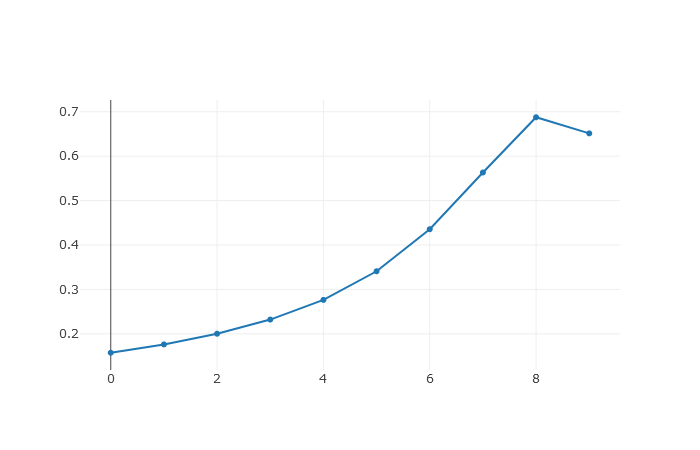
\includegraphics[scale=0.4]{newplot.png}

\pagebreak

Here is a plot where $n=100$ \\
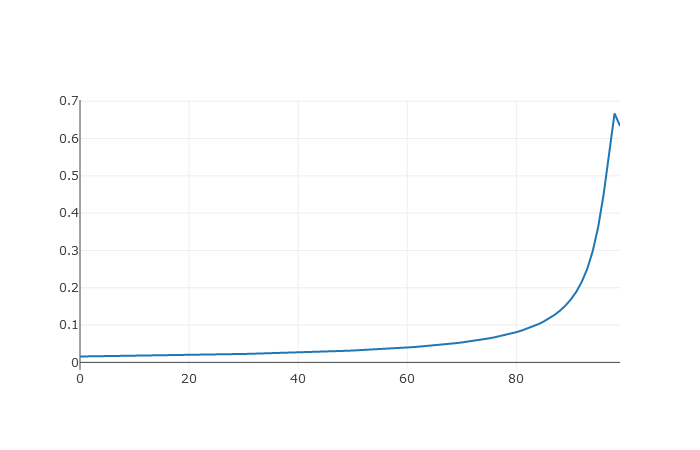
\includegraphics[scale=0.4]{100plot.png}

Here is the same plot, but the x axis (the lower boundary), only has values from 90 to 100 \\
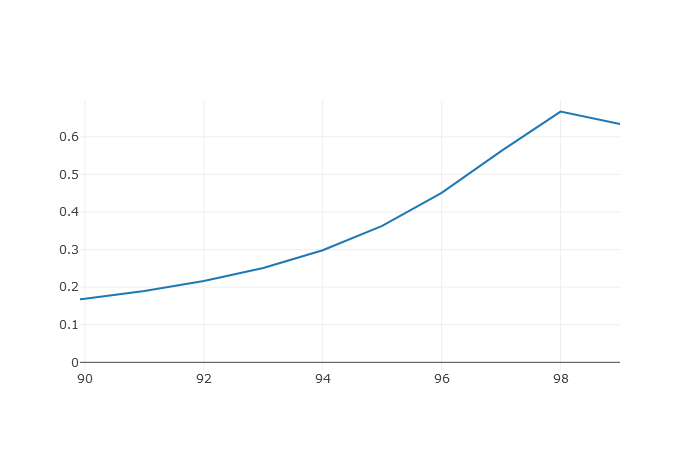
\includegraphics[scale=0.4]{90 100 plot.png}

\pagebreak

Here is a plot where $n=1000$ \\
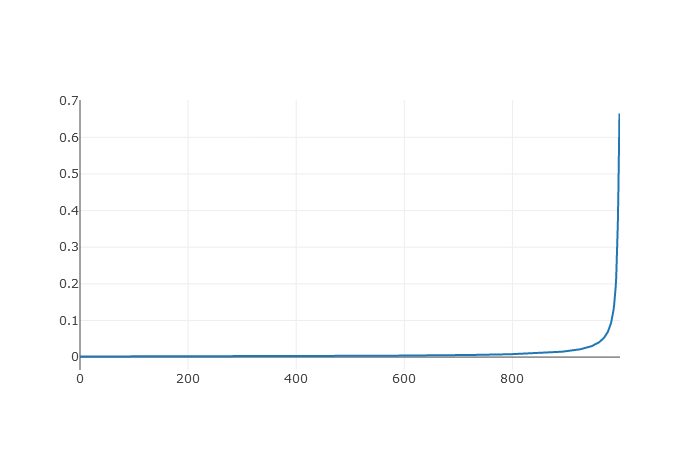
\includegraphics[scale=0.4]{1000 plot.png}

Here is the same plot, but the x axis (the lower boundary), only has values from 980 to 1000 \\
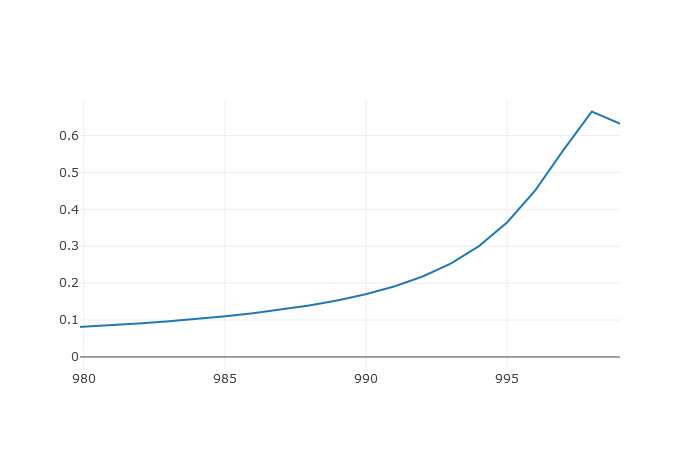
\includegraphics[scale=0.4]{980 1000 plot.png}

Observations: \\
The highest chance is always in the ballpark between 0.60 and 0.75 \\
The highest probabilty is always $n-2$, with n-1 being slightly lower. \\

\pagebreak

\subsection{Optimal Bound pick}
I sought to find out why $n-2$ was, in many cases of n with a uniform distribution, the optimal value of b (one that achieves the highest winrate.) I created a python script, which would iterate through different values of $n$ and check if $n-2$ was indeed the optimal bound pick. The program was able to prove this holds true for $n \in [2;1000] $ \\ I would have liked to prove this with the computer for $n \in [2;10000] $, but because of the time complexity, it would have taken years.


\subsection{'Average Biggest Box'}

The javascript simulation of the game calculated, over $10^5$ games, the average biggest amount of money in the $n$ boxes. For $n=10$, it computed that the 'average biggest box' was about 9,5. \\
The theoretical proof is as such:\\



P (10 dollars is highest)\\
= P (10 exists at least once in 10 boxes)\\
= $1-$P (10 does not exist at least once in 10 boxes)\\
\[
= \left( 1 - \left( \frac{9}{10} \right)^{10} \right) \cdot
\color{red} \left(\frac{10}{10}\right)^{10} \color{black}
\quad \approx 0,6513
\]
\\
\\
P(9 dollars is highest)\\
= P (9 dollars exists at least once in 10 boxes) AND P (10 dollars does not exist at least once in 10 boxes)\\
= $1-$P (10 dollars does not exist at least once in 10 boxes) AND P (9 dollars exists at least once in 10 boxes )\\
\[
= \left( 1 - \left(\frac{8}{9}\right)^{10} \right) \cdot \left(\frac{9}{10}\right)^{10}
\quad \approx 0,2413
\]
P(8 dollars is highest)\\
= P (8 dollars exists at least once in 10 boxes) AND P (10 and 9 dollars do not exist at least once in 10 boxes)\\
= $1-$P (10 and 9 dollars do not exist at least once in 10 boxes) AND P (8 dollars exists at least once in 10 boxes )\\
\[
= \left( 1 - \left(\frac{7}{8}\right)^{10} \right) \cdot \left(\frac{8}{10}\right)^{10}
\quad \approx 0,079
\]

etc...\\

We now need to take the average of each of these probabilities by multiplying them by the dollar value, and then dividing this total by the number of boxes, 10.
\[
\approx \frac{(0,651 \cdot 10) + ( 0,241 \cdot 9) + (8 \cdot 0,079) \textrm{  etc...  }}{10} \approx 9,5
\]
Or more mathematically \\ 
\[
\sum_{i=0}^{9} \left( \left(  1-\left(\frac{9-i}{10-i}\right)^{10} \right) \cdot \left(\frac{10-i}{10}\right)    ^{10}       \right) \left(10-i\right) = 9,5085
\]
We can generalize for $n$ boxes,
\[
x = \sum_{i=0}^{n-1} \left( \left(  1-\left(\frac{(n-1)-i}{n-i}\right)^{n} \right) \cdot \left(\frac{n-i}{n}\right)    ^{n}       \right) \left(n-i\right)
\]
So for:\\
$n=10$, $x=9,5085$\\
$n=100$, $x=99.4278$\\
A plot with $n$ on the x-axis and the average $x$ on the y-axis gives us:

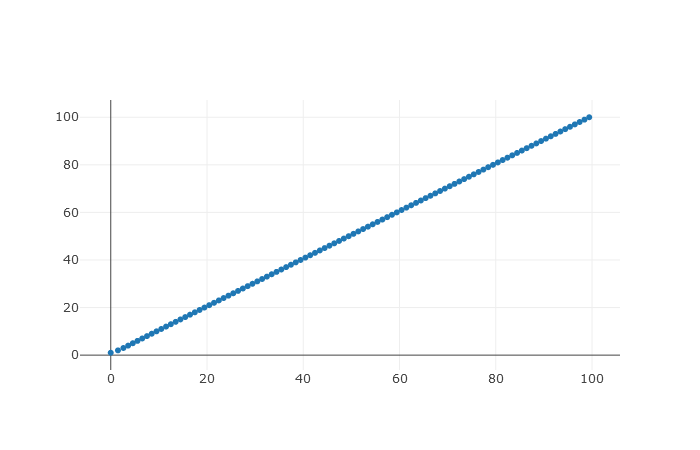
\includegraphics[scale=0.3]{average biggest box.png}


\section{Re-Evaluation}

The second strategy i considered, was what i called a re-evaluation strategy.\\ Instead of only taking into account the value inside the box, one also takes into account how many boxes the player has already opened. In essence, the player should take fewer risks if there are fewer boxes left. \\ \\
In this example, for a game with $n=10$ boxes, you lower the lower bound $b$ by 1 for every box you open after the 6th box.\\
This brought the winrate to $P = 71,69 \% $. \\
Further research could provide a theoretical proof for this strategy.



\section{Normal Distribution}

The next distribution of values i considered was a normal, or Gaussian distribution. In my javascript simulation, i added a function to simulate a Gaussian distribution of values, where one could specify the mean and standard deviation. The function is based on the Marsaglia polar method.\\
I randomized the standard deviation between 0,2 and 1 :\\ $\sigma \in [0,2;1]$\\
and the mean between 3 and 8 :\\ $ \bar{x} \in [3;8]$
On the following graph, the x-axis is the lower boundary $b$, and the y-axis is the probability of winning $P$, for $n=10$

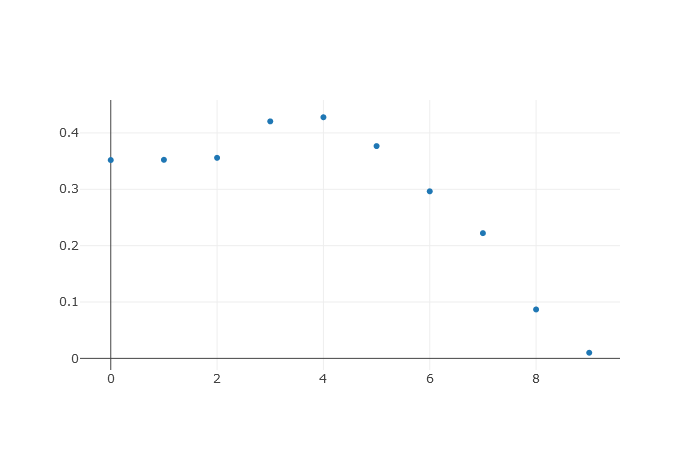
\includegraphics[scale=0.4]{normal10.png}

We can see that the scatter is quite a bit different than for the uniform distribution.\\ The best lower boundary is 4, where we get a probability of $P=43,78 \%$

\subsection{Cheeky Strategy}

I wanted to create a strategy that takes into account not only the value of the current box and amount of previous boxes, but also the values inside previous boxes.\\
Looking at past boxes could give an indication of the values inside the boxes to come.\\
 The algorithm is tailored to a normal distribution.\\
  It first opens half of all the boxes, and logs the values inside of them. It then checks what the average of these boxes is, and how many boxes are 1 dollar away drom this average.\\
 Based on this information, it decides how much risk to take.\\
  If between 0/5 and 1/5 of the boxes opened were more than 1 dollar away from the average, it would take the next box after having opened half.\\
  If between 1/5 and 2/5 of the boxes opened were more than 1 dollar away from the average, it would take the next box that had 1 dollar more than the average.\\
 If between 2/5 and 3/5 of the boxes opened were more than 1 dollar away from the average, it would take the next box that had 2 dollars more than the average.\\
  If between 3/5 and 5/5 of the boxes opened were more than 1 dollar away from the average, it would take the next box that had 3 dollars more than the average.\\ \\
  
  Ultimately, this strategy was unfortunately not better than the lower bound pick strategy.
  \color{red}$P = 42,66 \%$ \color{black}
  \\ \\
  In further research, one could calculate the mean and standard deviation for a certain amount of boxes, and decide how many dollars to take based on those variables.
  
  \pagebreak
  
\section{Random Distribution}

The final distribution, and ultimately the goal of the entire problem, is to find a strategy for the 'random' distribution.\\ I created a function which took 9 elements from $\in [0,1]$. \\
I called them $x_1,x_2,x_3...$
Then, i created the variable $u$,   $\in [0;1]$  \\
If\\
$u \in [0,x_1] \rightarrow 1$\\
$u \in [x_1,x_2] \rightarrow 2$\\
$u \in [x_2,x_3] \rightarrow 3$\\
$u \in [x_3,x_4] \rightarrow 4$\\
etc...
If I do this with 10 different values of $u$,I would get a random distribution.
If i use the lower bound pick strategy, i will get a much lower winrate than with a uniform distribution of money. In fact, all the values are between$P=1,95\% and P=2,05\%$\\
The lower bound pick strategy is mostly worthless with a random distribution.\\

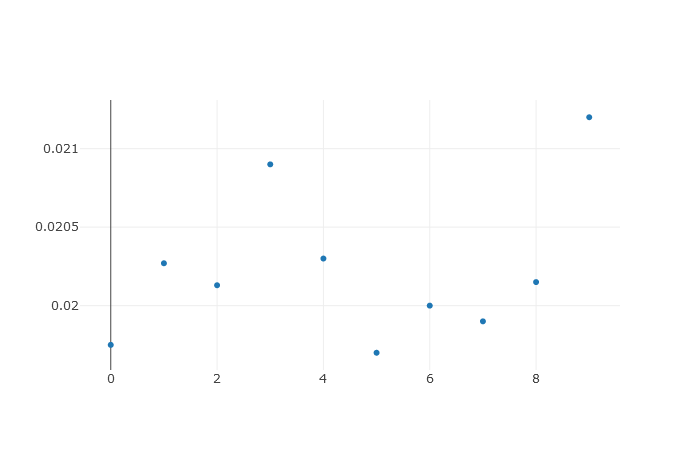
\includegraphics[scale=0.4]{random.png}

Further research could find a better strategy for this random distribution. 











\end{document}